
\section{Theorie}
\label{sec:Theorie}
\subsection{Das radioaktive Isotop}
Der Kern eines Atoms besteht aus Protonen und Neutronen. Dieser ist nur stabil, solange sich das Verhältnis beider innerhalb enger Grenzen befindet. Liegt es hingegen außerhalb der Grenzen ist der Kern instabil und zerfällt zu einem kleineren Kern. Das entsprechende Atom ist dann radioaktiv. Die Wahrscheinlichkeit mit welcher ein Kern innerhalb eines Zeitintervalls wird über seine Halbwertszeit $\tau$ definiert, nach welcher die Hälfte der Kerne zerfallen sind.

\subsection{Die Kernreaktionen mit Neutronen}
Dringt ein freies Neutron in den Wechselwirkungsbereich eines Kerns K ein, wird es von letzterem absorbiert. Der neue Kern K* wird als Compoundkern bezeichnet und liegt energetisch um die Gesamtenergie des Neutrons höher. Die zusätzliche Energie verteilt sich über die Nukleonen des Kerns und hebt diese in höhere Niveaus. Aufgrund der Energieverteilung besitzen die einzelnen Nukleonen nun zu wenig Energie, um das neue Neutron wieder abzustustoßen und geben die überschüssige Energie nur in Form von Gammaquanten wieder ab. Der neue Kern ist nun nicht mehr stabil und wandelt sich unter Abgabe eines Elektrons $\beta^-$ und eines Antineutrinos $\overline{\nu_\text{e}}$ in einen stabilen Kern um.
\begin{equation}
  \ce{^{m+1}_{z}A} \rightarrow \ce{^{m+1}_{z+1}C} + \beta^-  + E_\text{kin} + \overline{\nu_\text{e}}
\end{equation}
 Die nun überschüssige Energie geht in kinetische Energie von Elektron und Antineutrino über.


Die Wahrscheinlichkeit, mit welcher ein Kern ein freies Neutron fängt wird über den Wirkungsquerschnitt $\sigma$ dargestellt. Dieser beschreibt die Fläche, die ein theoretischer Kern besitzen müsste um jedes Neutron zu fangen. Für ihn gilt:
\begin{equation}
  \sigma = \frac{u}{n K d}\text{, }
\end{equation}
mit der Neutronenanzahl $n$, der Einfänge $u$ auf einer $\SI{1}{\square\centi\meter}$ großen Folie der Dicke $d$ und $K$ Atomen pro $\si{\cubic\centi\meter}$.
 Es zeigt sich jedoch , dass zwischen langsamen und schnellen Neutronen unterschieden werden muss. Ist die Geschwindigkeit des Neutrons groß, so ist die de-Broglie Wellenlänge des Neutrons klein gegenüber dem Kern und das Problem kann rein geometrisch betrachtet werden. Ist sie jedoch gering, so rücken die quantenmechanischen Effekte in den Vordergrund. In Näherung kann
 \begin{equation}
   \sigma = \frac{1}{v}
 \end{equation}
 angenommen werden, welches mit der Vorstellung übereinstimmt, dass sich ein langsames Neutron länger im Wirkungsbereichs des Kerns aufhält. Somit steigt die Wahrscheinlichkeit, dass die Kernkräfte es in den Kern ziehen.
 \subsection{Erzeugung langsamer Neutronen}
 Um die benötigten Neutronen zu gewinnen werden $^9$Be-Kerne mit der Alphastrahlung einer $^{226}$Ra Quelle beschossen. Dabei gilt:
\begin{equation}
  \ce{^{9}_{4}Be} + \ce{^{4}_{2}\alpha} \rightarrow \ce{^{12}_{6}C} + \ce{^{1}_{0}n}
\end{equation}
 Die entstandenen Neutronen besitzen eine kontinuierliches Energiespektrum bis zu $\SI{13.7}{\mega\electronvolt}$. Um sie auf die gewünschte mittlere kinetische Energie von $\SI{0.025}{\electronvolt}$ zu bringen, diffundieren sie vor dem Probenkontakt durch dicke Materieschichten, in welchen sie ihre kinetische Energie in elastischen Stößen abgeben. Die Stöße sind am effektivsten, wenn der Stoßpartner Wasserstoff ist. Wenn die Neutronen die Probe erreichen bewegen sie sich im Mittel nur noch mit $\SI{2.2}{\kilo\meter\per\second}$. Solche Neutronen werden als thermische Neutronen bezeichnet.
 \subsection{Der Zerfall instabiler Isotope}
 Ein instabiles Isotop zerfällt wie bereits beschrieben in stabile, leichtere Isotope. Für die Anzahl der zum Zeitpunkt $t$ noch nicht zerfallenen Kerne gilt dabei:
 \begin{equation}
   N(t) = N_0 e^{-\lambda t}\text{,}
   \end{equation}
mit den anfänglichen Kernen $N_0$ und der Zerfallskonstante $\lambda$.
Für $\tau$ folgt:
\begin{equation}
  \tau = \frac{\log(2)}{\lambda}\text{.}\label{T}
\end{equation}
Die zur Zeit $t$ noch existierenden Kerne zu bestimmen ist jedoch sehr schwierig.
Deswegen werden stattdessen die auftretenden Zerfälle in einem festen Zeitintervall gemessen, da diese ebenso exponentiell mit der Zeit abfallen. Für sie gilt:
\begin{equation}
  N_{\Delta t}(t) = N_0 \left(1 - e^{-\lambda \Delta t}\right)e^{- \lambda t} \text{  bzw.  } \ln \left( N_{\Delta t}(t) \right) = \ln \left( N_0(1- e^{- \lambda \Delta t}) \right) - \lambda t \text{,}
\end{equation}
wobei letzteres eine lineare Funktion darstellt.
Es ist jedoch darauf zu achten geeignete Zeitintervalle zu verwenden, damit die statistischen Fehler gering bleiben, jedoch auch keine systematischen Fehler auftreten.
Auf diese Weise kann das Zerfallsverhalten vieler Stoffe untersucht werden. Für das Element Indium gilt beispielsweise:
\begin{equation}
  \ce{^{115}_{49}In} +n \rightarrow \ce{^{116}_{49}In} \rightarrow \ce{^{116}_{50}Sn} + \beta^- + \overline{\nu_\text{e}}
\end{equation}\\
Es gibt jedoch auch einige Sonderfälle, von denen der Fall Rhodium nun gesondert betrachtet wird.
Bei der Aktivierung von reinem $^{103}$Rh durch Neutronen können nach der Zerfallsreihe in \eqref{jabadaba}
zwei verschiedene Isomere entstehen, welche sich in ihrer Energie unterschieden. Das langlebige $^{104i}$Rh zerfällt anschließend wieder zu energieärmeren $^{104}$Rh.
Das verwendete Zählrohr zählt jedoch die Zerfälle beider Reihen. Aufgrund der sehr unterschiedlich Halbwertszeiten kann jedoch davon ausgegangen werden, dass das kurzlebige Isomer nach einiger Zeit zerfallen ist und von da an nur noch Zerfälle des langlebigen registriert werden. Zwar zerfällt auch das durch den $^{104i}$Rh- Zerfall entstandene $^{104}$Rh weiter zu $^{104}$Pd, jedoch spielen diese Zerfälle nur eine untergeordnete Rolle.
\begin{equation}
  \ce{^{103}_{45}Rh}
\begin{cases}
   \stackrel{10\%}{\rightarrow} \ce{^{104i}_{45}Rh} \rightarrow \ce{^{104}_{45}Rh} + \gamma \rightarrow \ce{^{104}_{46}Pd} + \beta^- + \overline{\nu_\text{e}}\\
   \stackrel{90\%}{\rightarrow}  \ce{^{104}_{45}Rh} \rightarrow \ce{^{104}_{46}Pd} + \beta^- + \overline{\nu_\text{e}}\\
\end{cases}\label{jabadaba}
\end{equation}
%\begin{figure}
 %\centering
 %\caption{Die Neutronenaktivierung von $^{103}$Rh \cite{V702}}
 %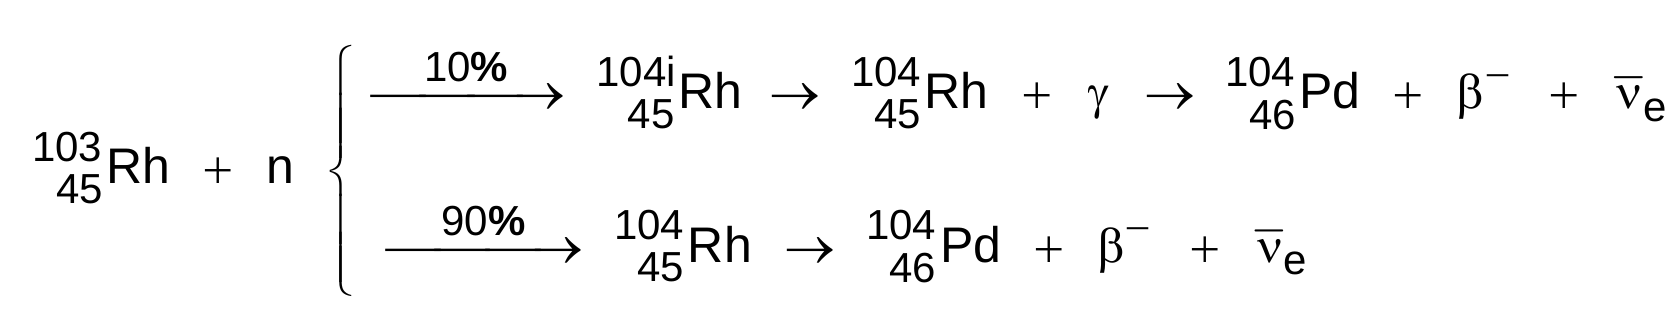
\includegraphics[width=\linewidth-150pt,height=\textheight-150pt,keepaspectratio]{content/rhodium.png}
 %\label{fig:rod}
%\end{figure}
